%% LyX 1.6.0 created this file.  For more info, see http://www.lyx.org/.
%% Do not edit unless you really know what you are doing.
\documentclass[english]{beamer}
\usepackage{mathptmx}
\usepackage[T1]{fontenc}
\usepackage[latin9]{inputenc}
\usepackage{amsmath}
\usepackage{amssymb}

\makeatletter
%%%%%%%%%%%%%%%%%%%%%%%%%%%%%% Textclass specific LaTeX commands.
 % this default might be overridden by plain title style
 \newcommand\makebeamertitle{\frame{\maketitle}}%
 \AtBeginDocument{
   \let\origtableofcontents=\tableofcontents
   \def\tableofcontents{\@ifnextchar[{\origtableofcontents}{\gobbletableofcontents}}
   \def\gobbletableofcontents#1{\origtableofcontents}
 }
 \makeatletter
 \long\def\lyxframe#1{\@lyxframe#1\@lyxframestop}%
 \def\@lyxframe{\@ifnextchar<{\@@lyxframe}{\@@lyxframe<*>}}%
 \def\@@lyxframe<#1>{\@ifnextchar[{\@@@lyxframe<#1>}{\@@@lyxframe<#1>[]}}
 \def\@@@lyxframe<#1>[{\@ifnextchar<{\@@@@@lyxframe<#1>[}{\@@@@lyxframe<#1>[<*>][}}
 \def\@@@@@lyxframe<#1>[#2]{\@ifnextchar[{\@@@@lyxframe<#1>[#2]}{\@@@@lyxframe<#1>[#2][]}}
 \long\def\@@@@lyxframe<#1>[#2][#3]#4\@lyxframestop#5\lyxframeend{%
   \frame<#1>[#2][#3]{\frametitle{#4}#5}}
 \makeatother
 \def\lyxframeend{} % In case there is a superfluous frame end

%%%%%%%%%%%%%%%%%%%%%%%%%%%%%% User specified LaTeX commands.
\usetheme{Warsaw}
% or ...

\setbeamercovered{transparent}
% or whatever (possibly just delete it)

\makeatother

\usepackage{babel}

\begin{document}

\title{Elliptic Curve Cryptography}


\author{G. Aleksandrowicz\inst{1} \and B. Hess\inst{2}}


\institute{\inst{1}Department of Computer Science, Technion \and \inst{2} Department of Computer Science, ETH Zurich}


%\date{Technion - Israel Institute of Technology\and \inst{2}Department
%of Theoretical Philosophy}


%\date{University of Else}


\date{Project in Computer Security, 2009}

\makebeamertitle

\lyxframeend{}\lyxframe{Outline}

\tableofcontents{}




\lyxframeend{}\section{Public Key Cryptosystems}

\lyxframeend{}\lyxframe{Familiar Cryptosystems}
\begin{itemize}
\item Diffie-Hellman key exchange
\item RSA cryptosystem.
\item El-Gamal cryptosystem.
\item Rely on hardness of factoring/discrete logarithm in $\mathbb{Z}_{n}^{*}$.
\item Typical key size of around 2048 bits.
\end{itemize}

\lyxframeend{}

\lyxframe{Enter Elliptic Curves}
\begin{itemize}
\item Elliptic Curves provide a wide variety of groups, similar to $\mathbb{Z}_{n}^{*}$
but more complex.
\item Diffie-Hellman and El-Gamal can be reproduced in this setting.
\item The discrete logarithm problem is much harder - i.e. the index calculus
method is not applicable.
\item This results in much smaller key sizes (100-200 bits).
\item The problem: More costly to generate, more costly to operate.
\end{itemize}

\lyxframeend{}
\lyxframe{Equivalent Key Sizes}
\begin{itemize}
 \item Equivalent secure key sizes for: Symmetric cryptography (AES), traditional PKC (RSA/DH) and ECC:
\end{itemize}

\begin{table}
% use packages: array
\begin{tabular}{c|c|c}
AES & $\mathbb{Z}_{n}^{*}$ PKC & ECC \\ \cline{1-3}
80 & 1024 & 160 \\ 
112 & 2048 & 224 \\ 
128 & 3072 & 256 \\ 
192 & 7680 & 384 \\ 
256 & 15360 & 521
\end{tabular}
\caption{Equivalent key sizes in bits, recommended by NIST}
\end{table}


\lyxframeend{}\section{Elliptic Curves}


\lyxframeend{}

\lyxframe{Definition}


\begin{itemize}
\item An Elliptic Curve is the set of solutions of an equation of the form
$y^{2}=x^{3}+ax+b$ over some field $\mathbb{F}$.
\item Usually denoted $E_{\mathbb{F}}$.
\item There is a small condition on $a,b$ ($4a^{3}+27b^{2}\ne0$)
\item If $\mbox{char}\mathbb{F}=2,3$ the equation is a little more complex...
\item We also consider a solution {}``at infinity'', $O$.
\end{itemize}

\lyxframeend{}\lyxframe{The Group Operation}
\begin{itemize}
\item Given points $P,Q\in E$ on the curve, we define $P+Q$ in the following
strange way:
\item Draw a line between $P,Q$. This line intersects the curve at another
point (or infinity). Take the reflection of that point relative to
the $x$-axis to be $P+Q$.
\item If $P=Q$ draw the line tangent to the curve at $P$. It intersects
the curve at one other point (or infinity).
\item For all $P$, $P+O=P$.
\item Motivation for such a stange definition: exists, and is derived from
the behivour of elliptic curves over $\mathbb{C}$. We cannot go into
details here.
\item This operations make $E$ into an abelian group.
\end{itemize}

\lyxframeend{}\lyxframe{The Group Operation - Illustration}
\begin{figure}[h]
\centering
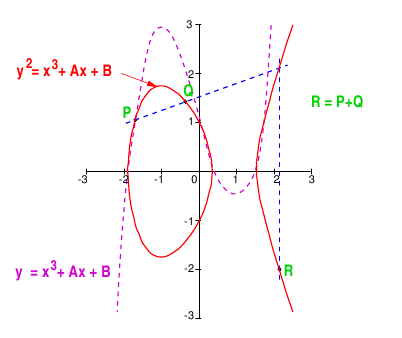
\includegraphics[scale=0.4]{ecaddition.png}
\caption{Addition of two points $P+Q$ in an EC}
\label{tradebefore}
\end{figure}

\lyxframeend{}\lyxframe{Group Operations in Practice}
\begin{itemize}
\item Given $E$ over $\mathbb{F}$ such that $\mbox{char}\mathbb{F}$ and
$P_{1}=\left(x_{1},y_{1}\right),P_{2}=\left(x_{2},y_{2}\right)$ ($P_{1}\ne\pm P_{2}$)
we can describe $P_{3}=P_{1}+P_{2}$ by:\end{itemize}
\begin{fact}%{}
$x_{3}=\left(\frac{y_{2}-y_{1}}{x_{2}-x_{1}}\right)^{2}-x_{1}-x_{2},y_{3}=\left(\frac{y_{2}-y_{1}}{x_{2}-x_{1}}\right)\left(x_{1}-x_{3}\right)-y_{1}$\end{fact}%{}
\begin{itemize}
\item If $P_{1}=P_{2}$ we have for $P_{3}$:\end{itemize}
\begin{fact}%{}
$x_{3}=\left(\frac{3x_{1}^{2}+a}{2y_{1}}\right)^{2}-2x_{1},y_{3}=\left(\frac{3x_{1}^{2}+a}{2y_{1}}\right)\left(x_{1}-x_{3}\right)-y_{1}$\end{fact}%{}
\begin{itemize}
\item Proof: Basic analytic geometry.
\end{itemize}

\lyxframeend{}\lyxframe{Group Operations with Projective Coordinates}
\begin{itemize}
\item Addition is costly, requires computing the inverse
\item Do computation in coordinate system where this can be avoided
\item Jacobian coordinates: $(X,Y,Z)$ corresponds to $(X/Z^2,Y/Z^3)$
\item Costs using jacobian coordiantes:
\begin{itemize}
 \item Doubling: 4 multiplications, 4 squarings
 \item Addition: 8 multiplications, 3 squarings
\end{itemize}
\item Multiplication of point $P$ with scalar $k$ is dominant operation.
\begin{itemize}
 \item Using with repeated doubling where possible.
\end{itemize}

\end{itemize}

\lyxframeend{}\section{Elliptic Curve Cryptosystems}

\lyxframeend{}\lyxframe{EC Key Pair Generation}
Public Parameters:
\begin{itemize}
\item An elliptic curve $E(\mathbb{F}_p)$
\item A curve-point $P$, which generates a cyclic subgroup of $E$, of order $n$:
\begin{fact}
 $\langle P\rangle=\{\infty,P,2P,3P,...,(n-1)P\}$
\end{fact}
\end{itemize}

Algorithm:
\begin{enumerate}
 \item Choose $d\in_{u.a.r.}\{1,...,n-1\}$
 \item Compute $Q=dP$
 \item Output pair $(Q,d)$. public key: $Q$, private key: $d$
\end{enumerate}

\lyxframeend{}\lyxframe{EC El-Gamal}
Public Parameters:
\begin{itemize}
\item Elliptic curve $E(\mathbb{F}_p)$, point $P$, order $n$
\item A public key $Q$.
\end{itemize}

Algorithm (encrypting message $m$)
\begin{enumerate}
\item Map $m$ to a point in $E$, let's say to $M$
\item Choose $k\in_{u.a.r.}\{1,...,n-1\}$ (\textcolor{red}{non-determinism})
\item Compute $C_1=kP$
\item Compute $C_2=M+kQ$
\item Output ciphertext: $(C_1,C_2)$
\end{enumerate}

Decryption requires private key $d$:
\begin{itemize}
\item $C_1-dC_2=M+kQ-\underbrace{dkP}_{=k(dP)=kQ}=M$
\end{itemize}

\lyxframeend{}\section{Elliptic Curve Generation}
\lyxframeend{}\lyxframe{Random Curves}
\begin{itemize}
\item Some ``good'' fixed curves are recommended and are available from NIST
\item Random curves provide ``better'' security than fixed ones
\begin{itemize}
 \item No precomputation can be done
 \item Equivalent to 11 bit longer key size for fixed curve ([HMCD03])
\end{itemize}
\end{itemize}

Approach:
\begin{itemize}
\item Select a large random prime $p$ for $\mathbb{F}_p$.
\item EC: $y^2=x^3+ax+b$. Task: select random pair $(a,b)$
\item Main security requirement: $|E(\mathbb{F}_p)|=k\cdot p$, $p$ large prime.
\item Why? to avoid application of generic DL algorithms.
\end{itemize}

\lyxframeend{}\lyxframe{Random Curves - Generation Methods (1)}
Random Approach
\begin{itemize}
\item Choose parameters randomly, until security requirements fit
\item Implies computing EC order:
\begin{itemize}
 \item Schoof's algorithm
 \item Satoh's algorithm (more efficient, but only with small field characteristic)
\end{itemize}
\item Satoh, combined with early abort strategy is efficient...
\begin{itemize}
 \item Literature: 5s for 163bit curve, on 750MHz CPU
\end{itemize}

\item ...but not trivial
\end{itemize}

\lyxframeend{}\lyxframe{Random Curves - Generation Methods (2)}
Complex Multiplication Approach
\begin{itemize}
\item Idea: generate curve for given EC order
\item Literature shows efficient implementation is possible
\item Approach not completely random (not all curves can be generated)
\item However not much loss of generality
\end{itemize}


\lyxframeend{}\lyxframe{Testing}
\begin{itemize}
\item We use the \emph{CppUnit} framework for unit-testing
\item Testing EC arithmetic: addition, multiplication, inversion
\begin{itemize}
 \item Testdata for NIST curves is available from the NSA
 \item Testing algebraic properties (e.g. $p^{ord(E)}=1$)
\end{itemize}
\item Testing the cryptosystem:
\begin{itemize}
 \item Encryption of arbitrary messages
 \item Decryption of given ciphertexts
\end{itemize}


\end{itemize}

\lyxframeend{}

\appendix

\lyxframeend{}\section*{Appendix}


\lyxframeend{}\subsection*{For Further Reading}


\lyxframeend{}\lyxframe{[allowframebreaks]For Further Reading}

\beamertemplatebookbibitems
\begin{thebibliography}{1}
\bibitem{HMV}D. Hankerson, A. Menezes, S. Vanstone. Guide to Elliptic
Curve Cryptography. Springer, 2004.
\bibitem{HMV}H. Baier, J. Buchmann. Generation Methods of Elliptic Curves. 2002.	\beamertemplatearticlebibitems

\end{thebibliography}

\lyxframeend{}
\end{document}
